\documentclass[tikz,border=5mm]{standalone}
\usepackage{amsmath}

\begin{document}
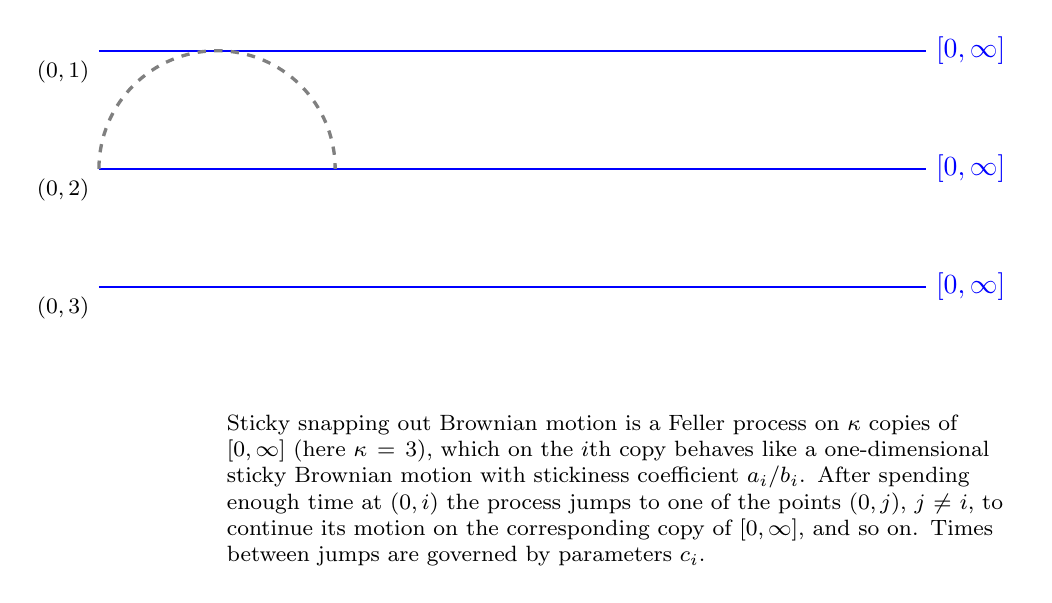
\begin{tikzpicture}[scale=1.5]

% Horizontal lines
\draw[blue, thick] (-1, 0) -- (6, 0) node[right] {$[0, \infty]$};
\draw[blue, thick] (-1, -1) -- (6, -1) node[right] {$[0, \infty]$};
\draw[blue, thick] (-1, -2) -- (6, -2) node[right] {$[0, \infty]$};

% Dotted semicircle
\draw[dashed, gray, very thick] (-1, -1) arc (180:0:1);

% Labels for the copies
\node[below left, font=\footnotesize] at (-1, 0) {$(0,1)$};
\node[below left, font=\footnotesize] at (-1, -1) {$(0,2)$};
\node[below left, font=\footnotesize] at (-1, -2) {$(0,3)$};

% Optional description (as per the provided caption)
\node[text width=10cm, align=left, below right, font=\footnotesize] at (0, -3) {
    Sticky snapping out Brownian motion is a Feller process on $\kappa$ copies of $[0,\infty]$ (here $\kappa = 3$), which on the $i$th copy behaves like a one-dimensional sticky Brownian motion with stickiness coefficient $a_i / b_i$. After spending enough time at $(0,i)$ the process jumps to one of the points $(0,j)$, $j \neq i$, to continue its motion on the corresponding copy of $[0,\infty]$, and so on. Times between jumps are governed by parameters $c_i$.
};

\end{tikzpicture}
\end{document}